\documentclass[conference]{IEEEtran}
\usepackage[T1]{fontenc}
\usepackage{graphicx,booktabs,amsmath,url,tikz}
\usetikzlibrary{arrows.meta,positioning}
\usepackage[hidelinks]{hyperref}
\title{A Four Lane SIMD Vector Processing Unit\\Phase I Design and Evaluation}
\author{\IEEEauthorblockN{Aanya Mehrotra \quad Vachan Gupta \quad Aditya Srivastava \quad Abhay}}
\begin{document}
\maketitle
\begin{abstract}
This project implements a single-instruction, multiple-data (SIMD) processing unit in Verilog. Four independent 8-bit arithmetic and logic lanes execute a common operation on two 32-bit vectors. A four-entry vector register file and a synchronous controller provide operand capture, execution and result writeback. Operations include addition, subtraction, AND, OR and unsigned less-than comparison. A scalar baseline reuses one ALU across four elements through the same host interface. Six self-checking testbenches verify components, integrated processors and matched workloads. The ALU passes 524,317 checks, SIMD integration passes 1,678 checks, and scalar integration passes 2,503 checks. Across 25 batches of 16 resident-vector instructions, SIMD completes in 47 elapsed cycles compared with 95 for scalar, giving a measured compute speed-up of 2.02. This report provides the architecture, microarchitecture, waveform evidence, target-specific synthesis and routed internal timing methodology, and a four-member contribution record.
\end{abstract}
\begin{IEEEkeywords}
SIMD, vector processing, Verilog, data-level parallelism, FPGA, verification
\end{IEEEkeywords}
\section{Introduction}
Independent array elements often require the same arithmetic or logic operation. Scalar hardware can process these sequentially, whereas a SIMD datapath applies one shared operation through multiple physical lanes. This project makes the distinction observable in a compact hardware model rather than a software-only timing analogy.

The objective is a modular four-lane prototype with explicit vector storage, reproducible verification and a comparable scalar design. The scope is four 8-bit unsigned elements per vector. It is a processing unit, not a complete instruction-fetching CPU. Phase I emphasizes the implemented prototype and evidence; the video is a separate deliverable.

\section{Literature Review}
Flynn classifies computer organizations by instruction and data streams, identifying SIMD as one instruction stream controlling multiple data streams~\cite{flynn}. This motivates the shared opcode and replicated lane ALUs. The prototype fixes the lane count and uses simple control so parallel activity can be inspected directly.

The RISC-V vector specification provides a contemporary reference for data-parallel execution, vector registers and configurable element widths~\cite{riscv}. Its mechanisms are substantially broader than this project. Here, vector width is 32 bits, the register file has four entries, and the operation set is deliberately small. The prototype does not implement the RISC-V ISA, configurable vector length, masking or vector memory instructions. The reference helps distinguish a demonstrator from a complete vector architecture.

Icarus Verilog separates compilation and elaboration from execution, enabling modular designs and reusable testbenches~\cite{icarus}. This supports exhaustive lane testing alongside directed and pseudorandom integration tests. Simulation establishes behavior under applied stimuli; synthesis and physical timing require additional tools. Yosys and nextpnr provide synthesis and FPGA place-and-route respectively~\cite{yosys,nextpnr}. They are used to obtain an explicit implementation target and measured resource and internal timing reports.

This project contributes an inspectable educational implementation with a controlled scalar comparison. It does not claim a new vector ISA or superiority over commercial vector processors.

\section{Proposed Solution}
\subsection{Architecture and Modules}
The SIMD top level connects a vector register file, operand and instruction capture registers, four combinational ALUs, result wiring and writeback multiplexers. Fig.~\ref{fig:arch} shows the datapath.
\begin{figure}[t]
\centering
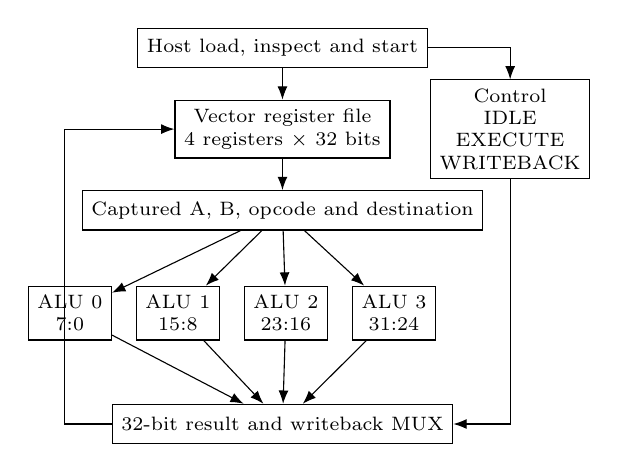
\begin{tikzpicture}[node distance=4mm, every node/.style={font=\scriptsize}, b/.style={draw,minimum height=5mm,align=center}, >=Latex]
\node[b] (host) {Host load, inspect and start};
\node[b,below=of host] (rf) {Vector register file\\4 registers $\times$ 32 bits};
\node[b,below=of rf] (cap) {Captured A, B, opcode and destination};
\node[b,below=7mm of cap,xshift=-27mm] (l0) {ALU 0\\7:0};
\node[b,right=3mm of l0] (l1) {ALU 1\\15:8};
\node[b,right=3mm of l1] (l2) {ALU 2\\23:16};
\node[b,right=3mm of l2] (l3) {ALU 3\\31:24};
\node[b,below=22mm of cap] (pack) {32-bit result and writeback MUX};
\node[b,right=5mm of rf] (ctrl) {Control\\IDLE\\EXECUTE\\WRITEBACK};
\draw[->](host)--(rf);\draw[->](rf)--(cap);
\foreach \l in {l0,l1,l2,l3} {\draw[->](cap)--(\l);\draw[->](\l)--(pack);}
\draw[->](pack.west)--++(-6mm,0)|-(rf.west);
\draw[->](host.east)-|(ctrl.north);
\draw[->](ctrl.south)|-(pack.east);
\end{tikzpicture}
\caption{SIMD datapath. One captured opcode controls all four ALUs. Result packing is wiring, not a reduction.}
\label{fig:arch}
\end{figure}

Lane 0 occupies bits [7:0], lane 1 [15:8], lane 2 [23:16] and lane 3 [31:24]. The register file has two asynchronous reads and one rising-edge write. Capturing source data, opcode and destination prevents later host input changes from altering an accepted operation. A destination may alias a source because operands are captured before writeback.

Opcodes 000, 001, 010, 011 and 100 select ADD, SUB, AND, OR and unsigned less-than. Reserved opcodes return zero. Addition and subtraction wrap modulo 256 within each lane; there is no inter-lane carry. Comparison returns an 8-bit zero or one rather than an all-ones mask.

\subsection{Control and Host Protocol}
Synchronous reset clears storage and control. While idle, host writes load a 32-bit vector at a rising edge if start is low. Start takes priority over a simultaneous host write. Writes and start requests while busy are discarded, not queued.

The SIMD controller follows IDLE $\rightarrow$ EXECUTE $\rightarrow$ WRITEBACK $\rightarrow$ IDLE. At E0 it captures an instruction. At E1 it enters WRITEBACK and asserts combinational write-enable. At E2 the register file samples that enable, stores the result and the controller pulses done. Elapsed acceptance-to-completion latency is two periods. The next acceptance can occur at E3, giving a three-period initiation interval. Reset during execution cancels work.

The inspection output shares read port A. With an idle start asserted, it shows source A; start must be low to inspect a selected register. Start held high until the next idle acceptance edge becomes a fresh request.

\subsection{Scalar Baseline}
The baseline shares storage, operations and host semantics but instantiates one ALU. It captures at E0, processes elements 0--3 at E1--E4, writes at E5 and accepts again at E6. Completion latency is five periods and initiation interval six. Capture and vector writeback overhead are included; the baseline is not claimed to be an optimized scalar CPU.

\section{Verification and Results}
\subsection{Functional Coverage}
All six Icarus testbenches pass (Table~\ref{tab:tests}). The lane sweep covers all $8\times256\times256$ opcode/input combinations plus 29 directed checks. Integration tests exercise distinct lane values, overflow, underflow, reserved opcodes, instruction capture, host arbitration, in-place writes and reset cancellation. Scalar reset tests cover each execution element and writeback.
\begin{table}[t]
\caption{Functional verification results}
\label{tab:tests}
\centering\small
\begin{tabular}{lr}\toprule
Testbench & Observed result\\\midrule
ALU lane & 524,317 checks, zero errors\\
Vector register file & PASS\\
Vector controller & PASS\\
SIMD integration & 1,678 checks, PASS\\
Scalar integration & 2,503 checks, PASS\\
Performance benchmark & 25 matched batches, PASS\\\bottomrule
\end{tabular}
\end{table}

Fig.~\ref{fig:wave} is generated from an actual simulator VCD. The directed ADD uses A=$\mathtt{FF800003}$ and B=$\mathtt{0180FF05}$. Result $\mathtt{0000FF08}$ comprises lane results 08, FF, 00 and 00 from low to high. The lanes operate on captured operands and a shared opcode; completion follows acceptance by two periods. The underlying VCD and generation script enable independent inspection.
\begin{figure*}[t]
\centering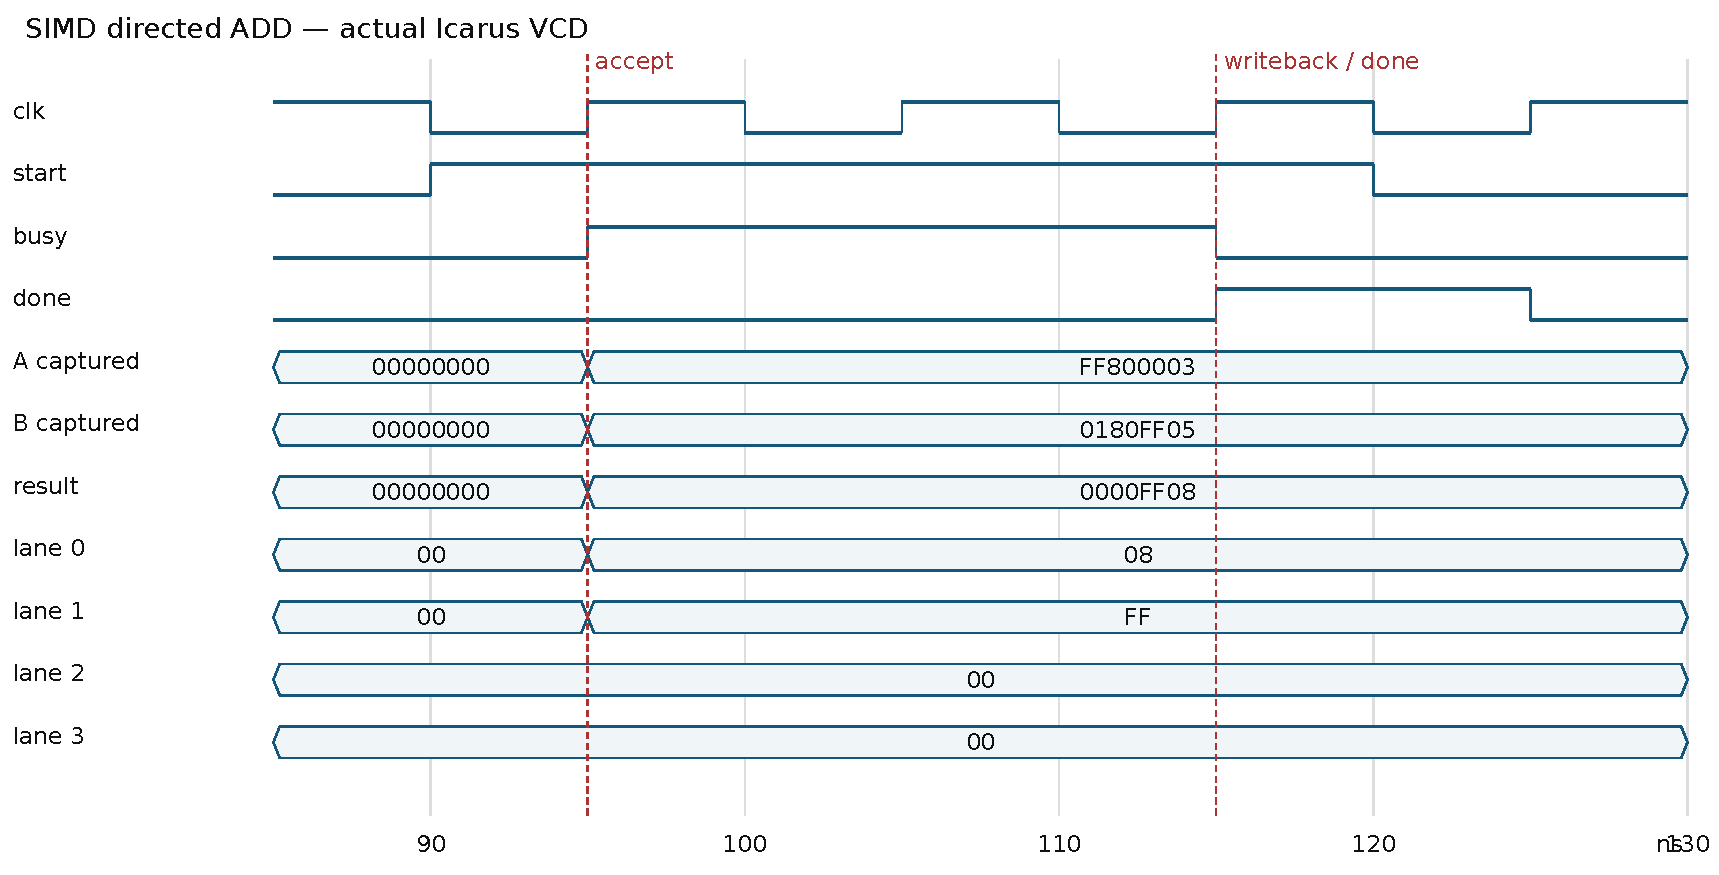
\includegraphics[width=\textwidth]{../evidence/simd_add_waveform.pdf}
\caption{Actual ADD waveform. Red markers identify acceptance and completion. Time is in ns.}
\label{fig:wave}
\end{figure*}

\subsection{Matched Workload and Performance}
Five operand pairs (one directed, four pseudorandom) are evaluated with all five valid operations. Each batch repeats 16 independent instructions on resident vectors, totaling 400 vectors per architecture across 25 batches. Every completed vector is checked against a reference model.

Timing spans the first accepted edge to final completion, excluding loading, inspection, software and external-memory overhead. For $N$ vectors:
\begin{equation}
C_{\mathrm{SIMD}}=3N-1,\qquad C_{\mathrm{scalar}}=6N-1.
\end{equation}
At $N=16$, measured counts are 47 and 95 periods:
\begin{equation}
S_{\mathrm{batch}}=95/47=2.021277.
\end{equation}
Single-instruction latency improves by $5/2=2.5$; steady-state throughput improves by two. SIMD sustains $4/3$ element operations per clock versus $4/6$ for this scalar baseline. These are distinct metrics, not a measured fourfold application speed-up.

\subsection{Synthesis and Routed Internal Timing}
Both top levels are independently synthesized with Yosys and placed and routed with nextpnr for a Lattice iCE40 HX8K in CT256, seed 1, with a 25\,MHz requested clock. Table~\ref{tab:fpga} is populated from mapped netlists and final routed clock reports.
\begin{table}[t]
\caption{Measured target-specific implementation results}
\label{tab:fpga}
\centering\scriptsize
\begin{tabular}{lrr}\hline Metric & SIMD & Scalar \\\hline
LUT4 cells & 427 & 347 \\
Flip-flop cells & 201 & 234 \\
Carry cells & 88 & 23 \\
Block RAM cells & 0 & 0 \\
Routed internal $f_{max}$ (MHz) & 114.1 & 82.86 \\
\hline\end{tabular}

\end{table}
Counts describe mapped primitive cells, not physical-board measurements. Pins are automatically placed; no board pinout or external input/output delay constraints are supplied. Reported $f_{\max}$ is the estimated routed internal clock limit under this setup, not board-level timing signoff. Simulation cycles and routed frequency are separate results. No hardware demonstration or power measurement is claimed.

\section{Individual Contributions}
The group has four members. The record below follows the repository's implemented areas and commit history.
\begin{itemize}
\item \textbf{Vachan Gupta:} ALU lane and directed and exhaustive testbench.
\item \textbf{Aditya Srivastava:} vector register file, controller and their tests.
\item \textbf{Aanya Mehrotra:} SIMD integration and verification, architecture and timing documentation, repository integration and Phase I packaging.
\item \textbf{Abhay:} scalar baseline and verification, matched workload benchmark, automated comparison and performance documentation.
\end{itemize}
ChatGPT assisted integration, verification, baseline development and documentation. The group is responsible for reviewing and understanding the submitted implementation.

\section{Conclusion}
The prototype demonstrates four-lane SIMD execution and a reproducible comparison with a one-ALU baseline. Measured batch speed-up is 2.02, reflecting capture and writeback overhead alongside parallel execution. Synthesis and routed internal timing complement functional evidence. Future work includes board-specific constraints, physical demonstration, more lanes and optional arithmetic operations. The video remains a separate submission deliverable.

\begin{thebibliography}{5}
\bibitem{flynn} M. J. Flynn, Some computer organizations and their effectiveness, \emph{IEEE Trans. Comput.}, vol. C-21, no. 9, pp. 948--960, Sep. 1972, doi: 10.1109/TC.1972.5009071.
\bibitem{riscv} RISC-V International, V standard extension for vector operations, version 1.0, \emph{Unprivileged ISA Specification}. [Online]. \url{https://docs.riscv.org/reference/isa/unpriv/v-st-ext}. Accessed: Nov. 14, 2026.
\bibitem{icarus} Icarus Verilog, Simulation using Icarus Verilog. [Online]. \url{https://steveicarus.github.io/iverilog/usage/simulation.html}. Accessed: Nov. 14, 2026.
\bibitem{yosys} YosysHQ, Yosys Open SYnthesis Suite. [Online]. \url{https://github.com/YosysHQ/yosys}. Accessed: Nov. 14, 2026.
\bibitem{nextpnr} YosysHQ, nextpnr portable FPGA place and route tool. [Online]. \url{https://github.com/YosysHQ/nextpnr}. Accessed: Nov. 14, 2026.
\end{thebibliography}
\end{document}
